\chapter{The sessions}

Each session correspond to a precise study case. When a new problem have to be analyzed, a new session has to be created.\\
%Chaque session correspond à un cas d'étude différent. Lorsque le logiciel est utilisé pour analyser une situation inédite, une nouvelle session doit être créée.\\

To make easier the comprehension of the different bricks, it is possible to personalize the name of actors. Those change will have an effect in only one session. 
%Une session est caractérisée par un ensemble d'acteurs plus ou moins importants (acteurs principaux et secondaires) et par les deux récits associés à chacun de ces acteurs. De plus, l'utilisateur donner un nom spécifique à chaque acteur afin de faciliter la compréhension des briques (ainsi, un acteur "père" peut être renommé en "M. X" au sein d'une session, ce renommage n'aura un impact qu'à l'intérieur de cette session).\\

\section{Session choice}
After launching \tria, the user have to choose one of these 3 options :\\
%Lors du lancement du logiciel, l'utilisateur est amené à choisir entre 3 options :\\
\begin{enumerate}
\item Edit all schemes : This is an automaticaly generated session. It correspond to the selection of all possibles actors, it allow the user to have a global view of all modelized situations.\\
%\item Editer l'ensemble des schémas : Cela correspond à une session générée automatiquement. Elle correspond à la sélection de tous les acteurs possibles. Cette session permet d'avoir une vue globale des situations schématisées dans le logiciel.
\item Create a new session : launch the session creation process.\\
%\item Créer une nouvelle session : Lance le processus de création d'une session.
\item Open a precedent session : The list of all precedent sessions is just bellow this option.\\
%\item Ouvrir une ancienne session : La liste des sessions précédentes se situe juste au dessous de cette option. Un double clique sur la ligne d'une ancienne session permet de l'ouvrir automatiquement.
\end{enumerate}

\begin{figure}[h!]
\centering
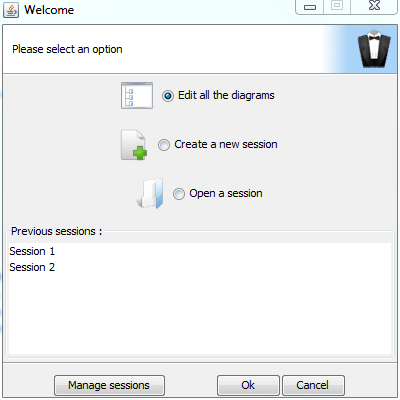
\includegraphics[scale=0.55]{images/ouverture_session.png}

\caption{The session choice wizard}
\end{figure}

\section{New session creation}
The first thing to do is to name the session. This could be with the "Session name" text field in the up of the window.\\
%La première chose à faire lors de la création d'une session est de nommer cette dernière. Cela se fait à l'aide du cadre "Nom de la session".\\

Then, the importants actors for the situation have to be selected. An actor could be selected as a main actor or a secondary actor. It could be changed later. You have to select the actor in the tree on the left and then click on one of the two buttons ("Add a main actor", "Add a secondary actor").\\
%Ensuite, il faut ajouter les acteurs concernés. Pour cela, il faut sélectionner un acteur dans l'arborescence située sur la gauche de la fenêtre puis cliquer sur un des boutons "Ajouter un acteur principal" ou "Ajouter un acteur secondaire". Il est toujours possible par la suite de changer le type d'un acteur sélectionné.\\

Somme things could be done on a selected actors : \\
%Lorsqu'un acteur a ainsi été ajouté, il apparaît dans la liste correspondante ("Acteurs principaux" ou "Acteurs secondaires"). Chaque ligne correspond à un acteur. Il est possible :\\
\begin{itemize}
\item delete the actor (with the little cross before its name)
%\item de supprimer l'acteur de la liste (petite croix juste avant le nom)
\item rename this actor for the session
%\item de renommer cet acteur pour la session
\item open its description (see section \ref{fiche_acteur})
%\item d'accéder à sa fiche (voir paragraphe \ref{fiche_acteur})
\item switch actor type (main or secondary)\\
%\item de changer le type de l'acteur (principal ou secondaire)\\
\end{itemize}



\begin{figure}[h!t]
\centering
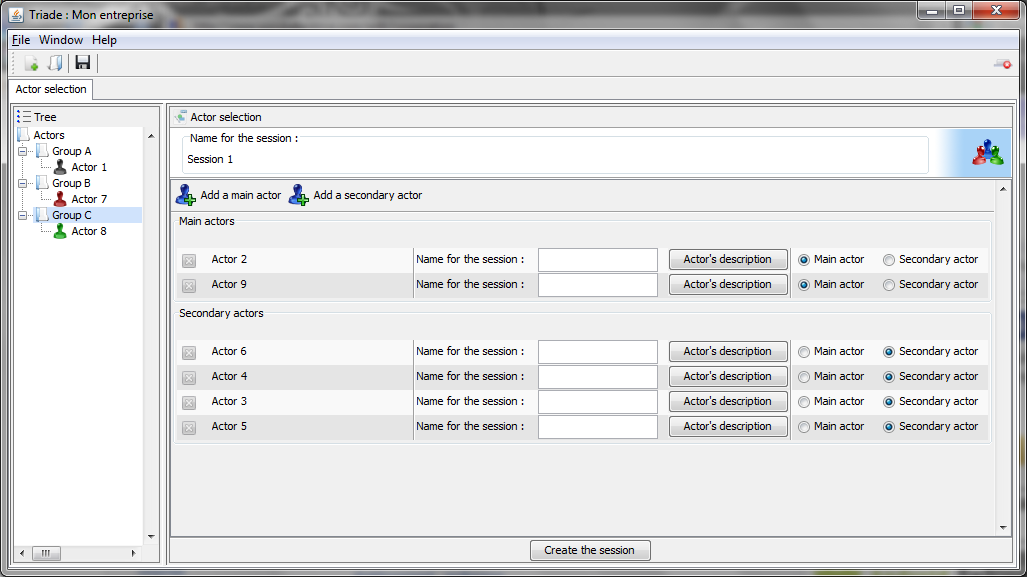
\includegraphics[scale=0.35]{images/selection_acteurs.png}

\caption{New session creation, the actor selection}

\end{figure}
The button "Create the session" on the bottom of the list create the session. Warning, the actor list can't be modified once the session has been created.\\
%Une fois la liste finalisée, il suffit de cliquer sur le bouton correspondant en bas de la fenêtre pour créer la session. Attention, il n'est plus possible de modifier la liste des acteurs une fois la session créée.\\

\section{Actor descriptions}
\label{fiche_acteur}
Each actor is associated to a description. It content the personalized name, the two tellings and a summry of the actor situations in the different brick. A description is linked two only one session.\\
%Chaque acteur est associé à une fiche. Elle permet de saisir les deux récits et de changer le nom associé à l'acteur. Chaque fiche est liée à une seule session (les récits saisis dans une session ne seront pas accessible depuis une autre). De plus un résumé de la situation de l'acteur est disponible à la suite des zones de texte.\\

You can get back the default name of an actor by deleting totally the personalized name.\\
%Il est possible de revenir au nom par défaut d'un acteur en supprimant complètement le texte dans le champ "Nom associé à l'acteur "..." pour la session".\\


%Les zones de textes "Premier récit", "Deuxième récit" et "Notes" permettent de saisir des %%%%%%%informations concernant cet acteur.\\
Bellow the text field, a section present a summary of the actors. The brick where this actor is present are sorted, first the brick with gapped relation, then the uncomplete ones and finally the corrects.\\
%La partie suivante présente un résumé de la situation de l'acteur, en triant les briques en fonctions des relations qui concernent cet acteur. En premier sont placés les briques présentant au moins une relation en écart, puis au moins une relation incomplète, et enfin celles n'ayant que des relations en accord. Il est possible d'accéder directement à une brique en cliquant sur son nom.\\

\begin{figure}[h!t]
\centering

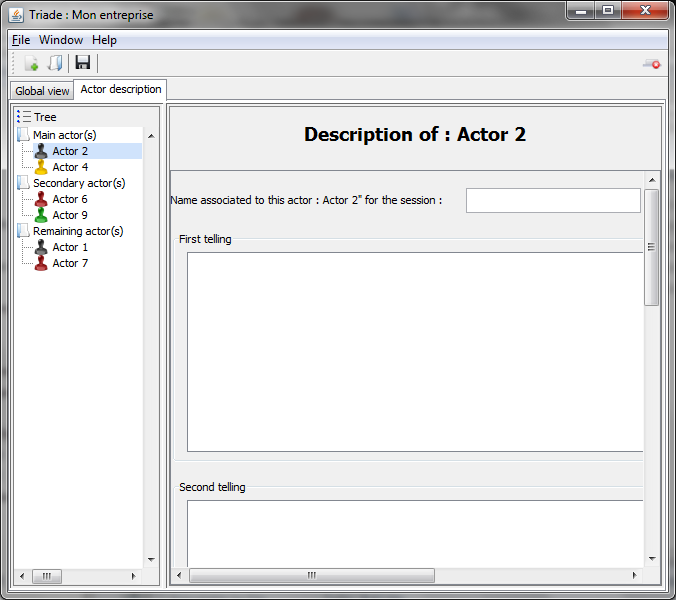
\includegraphics[width=12cm]{images/fiche_acteur.png}

\caption{An actor description}

\end{figure}
It is often possible to open an actor description by making a right click on the actor (in a tree or in a scheme). It's only not possible in an export window (see chapter \ref{export} about export).\\
%Il possible d'accéder à la fiche d'un acteur en faisant un clic droit sur ce dernier. Cela peut être fait dans un arbre ou dans une brique (voir figure~\ref{menu_fiche_acteur}). De plus l'arbre présent sur la gauche de la fiche d'un acteur permet d'accéder rapidement à l'ensemble des acteurs présent dans la sessions. La catégorie acteur restant correspond aux acteurs présent dans une brique mais n'ayant pas été sélectionné par l'utilisateur. Ces acteurs ne sont disponibles qu'une fois la session créée.\\

All the actor descriptions are opened in the tab "Actor list".\\
%L'onglet "Liste des acteurs" permet à tout moment de retourner à l'affichage des fiches des acteurs.


\begin{figure}[h!t]
\centering
\Ovalbox{
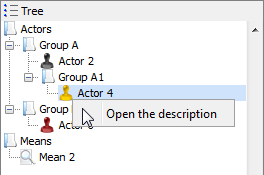
\includegraphics[width=6cm]{images/menu_fiche_acteur.png}
}

\caption{The contextual menu which give access to an actor description.}

\label{menu_fiche_acteur}
\end{figure}


\section{Session management interface}
The session management interface is accessible in the welcome panel with the "Manage sessions" button. It allows to manage current sessions with the following actions :\\
%Cette interface est accessible depuis l'écran d'acceuil de \tria. Elle permet de gérer l'ensemble des sessions courantes. Les actions possibles sont :\\
\begin{itemize}

\item \textbf{Open} : Open the selected session. If multiple sessions are selected, an error message is displayed.\\
%\item \textbf{Ouvrir} : Permet d'ouvrir la session sélectionné. Si plusieurs sessions sont sélectionnées, un message d'erreur apparaît.\\
\item \textbf{Archive} : Archive selected sessions in a file. Those sessions will be deleted from the current sessions list.\\
%\item \textbf{Archiver} : Permet d'enregistrer des sessions dans un fichier. Ces sessions sont ensuite supprimé de la liste des sessions courantes.\\
\item \textbf{Save as} : Save selected sessions in a file. The sessions are kept in the list.\\
%\item \textbf{Sauvegarder sous} : Permet d'enregistrer une copie des sessions sélectionnées dans un fichier. Ces sessions sont conservées dans la liste des sessions courantes.\\
\item \textbf{Import} : Add the sessions contained in an extern file to the current sessions list. If an existing session have the same name than one in the file, the software ask the user if he wants to keep the existing session or overwrite it with the one from the file. Warning, if the existing session is replaced, it will be lost.\\
%\item \textbf{Importer} : Permet d'ajouter à la liste des sessions courantes les sessions d'un fichier. Si une session portant le même nom qu'une session importée est déjà présente dans la liste, il sera demandé à l'utilisateur s'il veut remplacer la session présente dans la liste. Attention, en cas de remplacement, cette session sera perdue.\\
\item \textbf{Rename} : Allow to rename the selected sessions.\\
%\item \textbf{Renommer} : Permet de renommer les sessions sélectionnées. Il est possible de renommer plusieurs sessions à la suite en faisant une sélection multiple.\\
\item \textbf{Delete} : Delete selected sessions. Warning, this operation can't be undone.\\
%\item \textbf{Supprimer} : Permet de supprimer des sessions. Attention, cette opération est irréversible.
\end{itemize}

For multiple selection, use \textit{Ctrl} to add a session to the selection, and \textit{Shift} to select a group of sessions. This could be useful to archive or save a group of sessions in a same file.\\
%Il est possible de sélectionner plusieurs sessions en même temps afin d'exporter dans un même fichier un ensemble de sessions. Pour cela la touche \textit{Ctrl} permet d'ajouter un élément à la sélection, et \textit{Maj} permet de sélectionner un groupe de sessions.\\

\begin{figure}[h!]
\centering
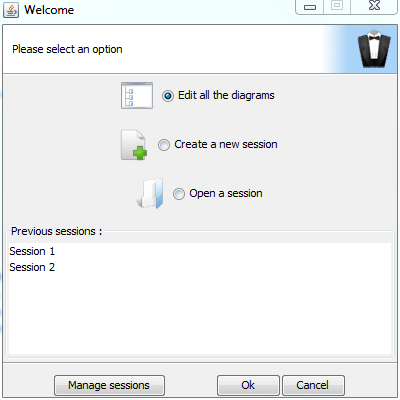
\includegraphics[width=0.6\textwidth]{images/ouverture_session.png}
\caption{The session management interface is accessible from the welcome panel}
\end{figure}

\begin{figure}[h!]
\centering
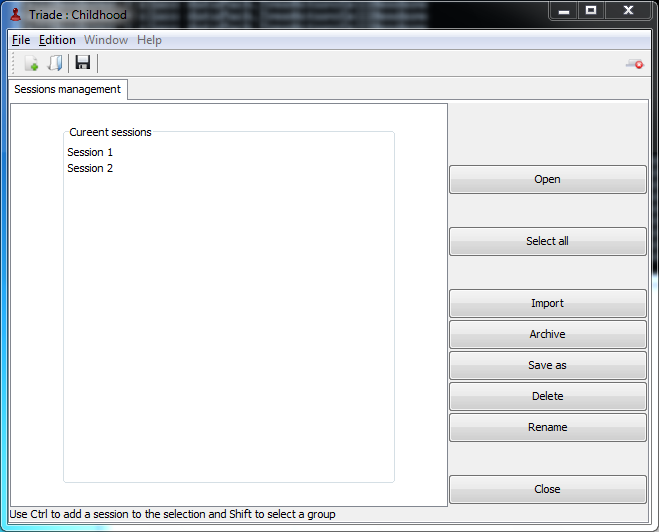
\includegraphics[width=0.8\textwidth]{images/gestion_session.png}
\caption{The session management interface}
\end{figure}
